\documentclass{exam}
 
 \usepackage{graphicx}
 \usepackage{float}
 \usepackage{amsmath}
 \usepackage{algorithm2e}
 \usepackage{algpseudocode}
 
% First we setup the header and footer
\pagestyle{headandfoot}
\runningheadrule
\runningfootrule
\header{CSE101: Design and Analysis of Algorithms (CSE, UCSD, Summer-2020)}{}{Homework-01}
\footer{}{\thepage  \, of \numpages}{}
 
% We want the points for each question displayed on the left
%\pointname{points}
%\pointsinmargin
 
% Automatically total the points - make sure to compile TWICE
\addpoints
 
\begin{document}


\begin{center} 
\fbox{\parbox{5.5in}{
\vspace{-0.1in}
\begin{itemize}
\item \small{For algorithm design questions, you may either give pseudocode or explain your algorithm using Mathematical English. You need to make sure that all steps of your algorithm are clear from your writeup. Even though we allow you the flexibility of expressing your algorithm in a paragraph, we would prefer if you give a pseudocode since it is a widely accepted format for expressing algorithms and it is easier to parse. }

\item \small{Please note that one of the main goals of this course is to design efficient algorithms. So, there are points for efficiency even though we may not explicitly state this in the question. }

\item \small{The other instructions are the same as in Homework-00.}
\end{itemize}
\vspace{-0.1in}
}}
\end{center}

\vspace{0.1in}


\vspace{0.1in}
% Some general text together with number of questions and total points possible
There are \numquestions\, questions for a total of \numpoints\, points.
\vspace{0.1in}
\hrule
 \vspace{0.2in}
\begin{questions}
 
% First question, worth 3 points
\question An undirected graph is said to be {\em connected} iff every pair of vertices in the graph are reachable from one another. Prove the following statement:
\begin{quote}
{\it Any connected undirected graph with $n$ nodes has at least $(n-1)$ edges.}
\end{quote}

We will prove the statement using Mathematical Induction. The first step in such a proof is to define the propositional function. Fortunately for this problem, this is already given in the statement of the claim. 

$P(n)$: Any connected undirected graph with $n$ nodes has at least $(n-1)$ edges.

The base case is simple. $P(1)$ holds since any connected graph with $1$ node having at least $0$ edges, is indeed true. 
For the inductive step, we assume that $P(1), P(2), ..., P(k)$ holds for an arbitrary $k \geq 1$, and then we will show that $P(k+1)$ holds. Consider any connected graph $G$ with $(k+1)$ nodes and $k$ edges. You are asked to complete the argument by doing the following case analysis:

\begin{parts}
\part[10] Show that if the degrees of all nodes in $G$ is at least $2$, then $G$ has at least $k$ edges.\\

Let $deg(G)$ denote $\sum_{v \in V} deg(v)$, the total sum of all degrees in a graph. If there are $k+1$ nodes in G, and all nodes in G have degree $\geq 2$, then $deg(G) \geq 2(k+1) = 2k+2$. Observe that when we add an edge into a graph, we connect 2 nodes, increasing the degrees of each connected node by one. This means that $deg(G)$ increases by 2 for every edge we add into a graph. If there are $E$ such edges, $deg(G) = 2 + 2 + 2 ...$ ($E$ times) $= 2E$. Simplifying, we get $E = \frac{deg(G)}{2} \geq \frac{2k+2}{2} = k + 1 > k$.\\

\part[10] Consider the case where there exists a node $v$ with degree $1$ in $G$. In this case, consider the graph $G'$ obtained from $G$ by removing vertex $v$ and its edge. Now use the induction assumption on $G'$ to conclude that $G$ has at least $k$ edges.\\

$G$ has $k + 1$ nodes and $k$ edges. We obtain $G'$ by removing vertex $v$ and its edge from $G$. This means $G'$ has $(k + 1) - 1 = k$ nodes and $k - 1$ edges. Using the induction assumption, it follows that $P(k + 1)$ must also hold on $G'$. Adding a node to a connected undirected graph requires the addition of at least one edge to maintain connectivity. Adding a node to $G'$, we get a graph with $k + 1$ nodes and $(k - 1) + 1 = k$ edges. Indeed, we see that adding a node to $G'$ results in $G$. We conclude that $P(k + 1)$ holds, and $G$ with $k + 1$ nodes has at least $k$ edges.\\
\end{parts}



\vspace{0.3in}




\question Consider the undirected graph given below and answer the questions that follow.
\begin{figure}[h]
\centering
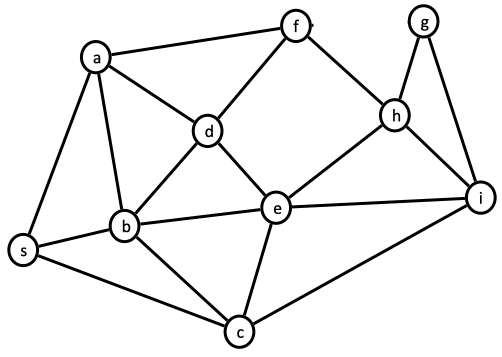
\includegraphics[scale=0.5]{G1}
\end{figure}

\begin{parts}
\part[5] Draw an adjacency list for the graph above. \\
({\it Note that the adjacency list may not be unique and hence there may be multiple correct answers to this part.})\\

A: B, D, F, S\\
B: A, C, D, E, S\\
C: B, E, I, S\\
D: A, B, E, F\\
E: B, C, D, H, I\\
F: A, D, H\\
G: H, I\\
H: E, F, G, I\\
I: C, E, G, H\\
S: A, B, C\\


\vspace*{0.1in}

\part[5] State the order in which the vertices of the graph get marked {\it visited} when {\tt explore($G, s$)} is executed. \\
({\it Please note that the answer to this part is dependent on your answer to part (a) since the order in which neighbors of a particular vertex $v$ are considered depends on the order of the neighbors in the linked list corresponding to $v$}.)\\

S, A, B, C, E, D, F, H, G, I\\

\vspace*{0.1in}



\part[5] State the order in which the vertices of the graph get marked {\it visited} when {\tt explore($G, h$)} is executed.\\
({\it As in part (b), the answer to this part depends on your answer to part (a).})\\

H, E, B, A, D, F, S, C, I, G
\end{parts}


\vspace{0.3in}


\question A {\it source} in a directed graph is a node that has no edges going into it. ({\it For example, the graph below has two source nodes, $A$ and $C$.})
\begin{figure}[h]
\centering
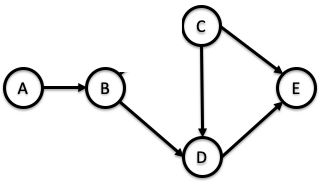
\includegraphics[scale=0.5]{source}
\end{figure}

Answer the questions below:

\begin{parts}
\part[15] Give a linear-time algorithm that takes as input a directed graph in adjacency list format, and outputs all of its sources. Discuss running time of your algorithm.\\

\begin{algorithm}
	\DontPrintSemicolon
	\SetKwFunction{FMain}{source}
	\SetKwProg{Fn}{procedure}{:}{}
	\Fn{\FMain{G}}{
		\ForAll(\tcp*[f]{O(V)}){v in V}{
			source[v] = true
		}
		\ForAll(\tcp*[f]{O(V)}){v in V}{
			\ForAll(\tcp*[f]{O(1 + deg(v)}){neighbor u of v}{
				source[u] = false
			}
		}
		L = empty list\\
		\ForAll(\tcp*[f]{O(V)}){v in V}{
			\If{source[v]}{
				add v to L
			}
		}
		\KwRet\ L
	}
\end{algorithm}

{\bf Analysis:}\\
Mark all nodes as sources. O(V)\\
For each node $v$ in $V$, mark its neighbors as non-sources, since each neighbor $u$ has an incoming edge from $v$ and cannot be a source. O(V + E)\\
Traverse through all the nodes, and return the set of all source nodes. O(V)\\
\\{\bf Time complexity:}\\
$O(V) + O(V+E) + O(V) = O(V + E)$\\

\part[5] Run your algorithm given in part (a) on the following directed graph given below and give the output.\\
\begin{tabular}{lllll}
A &: D & & &\\
B &: C, & D, & E & \tcp*[f]{Node B is the only source}\\
C &: F & & & \\
D &: E & & &\\
E &: A, & C & &\\
F &: I, & J & &\\
G &: A, & D, & K &\\
H &: D, & E, & G, & I\\
I &: J & & & \\
J &: C & & &\\
K &: H & & & 
\end{tabular}
\end{parts}



\vspace{0.3in}


\question[20] ({\it Fire safety}) The fire safety officer of a factory has a map of the factory which is an undirected graph $G = (V, E)$ where the nodes represent various factory locations and edges represent whether there is a fire-safe passage between locations. A set $S \subseteq V$ of locations in the factory are exit locations. The fire safety officer is interested in finding out whether people from all factory locations can be evacuated in case of a fire.

Design an algorithm for this problem. The input to your algorithm is  graph $G = (V, E)$ in adjacency list representation and a set $S \subseteq V$ of vertices. Discuss the running time of your algorithm.\\

\begin{algorithm}
	\DontPrintSemicolon
	\SetKwFunction{FMain}{escape}
	\SetKwProg{Fn}{procedure}{:}{}
	\Fn{\FMain{G}}{
		\ForAll(\tcp*[f]{O(V)}){v in V}{
			visited[v] = false
		}
		\ForAll(\tcp*[f]{O(V)}){s in S}{
			\If{not visited[s]}{
				explore(G, s) \tcp*{O(V + E)}
			}
		}
		\ForAll(\tcp*[f]{O(V)}){v in V}{
			\If{not visited[v]}{
				\KwRet\ false
			}
		}
		\KwRet\ true
	}
\end{algorithm}

{\bf Analysis:}\\
Mark all nodes as unvisited. O(V)\\
For each unvisited escape node $s$ in $S$, run DFS to mark all nodes reachable from $s$ as visited. Note that DFS will not run on visited escape nodes. O(V + E)\\
Traverse through all the nodes, and return if they have all been visited. O(V)\\
\\{\bf Time complexity:}\\
$O(V) + O(V + E) + O(V) = O(V + E)$\\

\newpage



\question Given a directed graph $G = (V, E)$ and a vertex $v \in V$, 
\begin{itemize}
\item let $S_v$ be a set that contain all the vertices that have a directed path to $v$ in $G$, and 
\item let $T_v$ be a set that contain all the vertices to which a directed path from $v$ in $G$ exists.
\end{itemize}
({\it For example, for the graph $G$ and vertex $A$ below, the set $S_A = \{A, B, C, D\}$ and $T_A = \{A, E\}$.})
\begin{figure}[h]
\centering
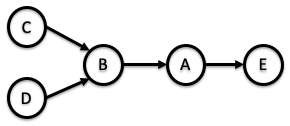
\includegraphics[scale=0.4]{reach}
\end{figure}



\begin{parts}
\part[10] Design an algorithm that takes as input a directed graph $G=(V, E)$ in adjacency list representation and a vertex $v \in V$, and outputs the set $(S_v \cap T_v)$ as defined above.

\begin{algorithm}
	\DontPrintSemicolon
	\SetKwFunction{FMain}{cycle}
	\SetKwProg{Fn}{procedure}{:}{}
	\Fn{\FMain{G, $v_0$}}{
		\ForAll(\tcp*[f]{O(V)}){v in V}{
			visited[v] = false, cycle[v] = false\\
		}
		STACK = empty stack of nodes\\
		ANS = empty set of nodes\\
		modifiedExplore(G, $v_0$, STACK, ANS) \tcp*[f]{O(V + E)}\\
		add $v_0$ to ANS\\
		\KwRet\ ANS
	}
\end{algorithm}

\begin{algorithm}
	\DontPrintSemicolon
	\SetKwFunction{FMain}{modifiedExplore}
	\SetKwProg{Fn}{procedure}{:}{}
	\Fn{\FMain{G, $v$, STACK, ANS}}{
		visited[v] = true\\
		PUSH v to STACK\\
		\ForAll(\tcp*[f]{1 + deg(v)}){neighbors u of v}{
			\If(\tcp*[f]{at most V times, once per v}){not visited[u]}{
				modifiedExplore(G, u)
			}
			\ElseIf{(u is $v_0$) or (cycle[u])}{
				\While(\tcp*[f]{bounded by recursive calls, at most V times}){STACK is not empty}{
					temp = POP STACK\\
					cycle[temp] = true\\
					add temp to ANS\\
				}
			}
		}
		POP STACK
	}
\end{algorithm}

\vspace{0.1in}

\part[10] Discuss running time of your algorithm.\\

{\bf Analysis:}\\
Mark all nodes as unvisited and not part of a cycle. O(V)\\
Create an empty recursion stack and empty answer set. O(1)\\
Run DFS on the target node $v_0$. Will not traverse nodes that are already visited. O(V + E)\\
If the DFS hits $v_0$ or a cycle containing $v_0$, pop all nodes from stack to answer set. Stack will only push unvisited nodes, so will only pop maximum of V times the entire procedure. O(V)\\

{\bf Time complexity:}\\
$O(V) + O(1) + O(V + E) + O(V) = O(V + E)$\\

\vspace{0.1in}

\part[5] Give proof of correctness of your algorithm.\\
\end{parts}

{\bf What is the question asking?}\\
The intersection of $S_v$ and $T_v$ contains all nodes that have a directed path {\em to} and {\em from} $v$ in $G$. If there is a directed path of node $u \rightarrow v$ and there is a directed path of node $v \rightarrow u$, the two nodes must be contained in the same cycle, since each node can reach itself through the path $u \rightarrow v \rightarrow u$. Therefore, $S_v \cap T_v$ contains all nodes that share a cycle with $v$.\\

We can find these nodes by running a DFS on $v$, and pushing every traversed element into a stack. Once our DFS hits $v$ again, we know that we have found a cycle, since our DFS found a directed path from $v \rightarrow ..... \rightarrow v$. From here, we pop all elements from the stack, and add them to our answer.\\

{\bf How do the nodes in the stack form a cycle with $v$?}\\
The first element we push to this stack will be $v$, since this is the element we first run DFS on. The next element we push to the stack, $element_{v+1}$, will be a direct neighbor to $v$, and thus there is a path from $v \rightarrow element_{v+1}$. Using induction, we can assume all elements in the stack form a path of $v \rightarrow element_{v+1} \rightarrow element_{v+2} \rightarrow ..... \rightarrow element_{top}$. Since a stack reverses the order of insertion when popping, all elements popped before (pushed after) $v$ will have a direct path in the form of $v \rightarrow element$.\\

Similarly, if the DFS detects back edge to $v$, there must also be a path from $element_{top} \rightarrow v$. Together, this guarantees we are returning the correct cycle, since $v \rightarrow element_{v+1} \rightarrow ..... \rightarrow element_{top} \rightarrow v$.\\

{\bf Which nodes are added to the stack?}\\
Elements will be added to the stack iff they are reachable from $v$. This means every element added to the stack is contained in $T_v$, since there is a path $v \rightarrow element$. However, this does not guarantee they are also contained in $S_v$. This property is checked later in the DFS call. Also, nodes cannot be added into the stack twice since DFS only traverses each node once.\\

{\bf When do we pop the right nodes from the stack to record them?}\\
Each iteration of DFS considers 3 possibilities:\\
1. The current node has unvisited neighbors. Recurse on them for future processing.\\
2. The current node has visited neighbors that are either $v$ or are part of a cycle that contains $v$. Functionally, these are the same, and both situations imply that the current node is contained in $S_v$, or there is a path of $element_{top} \rightarrow v$ (current node will be top element of stack). All elements in the stack are also contained in $T_v$. All elements in the stack form a cycle with $v$. Pop them from the stack to the answer set, and mark each popped node as part of a cycle.\\
3. The current node has visited neighbors that are not $v$ nor are part of a cycle that contains $v$. The node has been completely traversed, as guaranteed by DFS, and deemed a dead end. Do nothing, it will automatically be popped from the stack.\\

{\bf When do we pop the wrong nodes from the stack to discard them?}\\
Once the DFS has finished recursively processing a node, the node will be popped from the stack. All possible solutions involving the node have already been written to the answer set, so it is no longer under consideration. It is okay to pop an empty stack, as is the case when the current node has already been popped and written to the answer set.\\


\vspace{0.3in}







\end{questions}
\end{document}